\documentclass[times, 10pt]{article} 
%\documentclass[times, 10pt,twocolumn]{article} 
%\usepackage[noend]{distribalgo}
\usepackage{algorithm}
%\usepackage{times}
\usepackage{amsmath}
\usepackage{graphicx}
\usepackage{color}
\usepackage{amssymb}
\usepackage{xparse}
\usepackage[noend]{distribalgo}
\usepackage[draft]{fixme}
\usepackage[hmargin=2.5cm,vmargin=2.2cm]{geometry}


\begin{document}

\newcommand{\mv}[1]{\ensuremath{\operatorname{\mathit{#1}}}}
\definecolor{dark}{gray}{.6}
\newcommand{\bc}[1]{\textcolor{dark}{#1}}
\newtheorem{lems}{Lemma}
\newtheorem{props}{Proposition}
\newtheorem{thms}{Theorem}
\newtheorem{defs}{Definition}
\newtheorem{obs}{Observation}

\newcommand{\code}[1]{\texttt{\small{\textbf{#1}}}}

\newcommand{\blankline}{\vspace{4 mm}}
\newcommand{\amcast}{\mbox{multicast}}
\newcommand{\amdel}{\mbox{deliver}}
\newcommand{\amdelarg}[1]{\mbox{\amdel({#1})}}
\newcommand{\amcastarg}[1]{\mbox{\amcast({#1})}}
\newcommand{\tconsm}{T_{cons}}
\newcommand{\tcons}{\mbox{$\tconsm$}}
\newcommand{\opt}{\mbox{opt-deliver}}
\newcommand{\cons}{\mbox{deliver}}
\newcommand{\rmcast}{\mbox{r-mcast}}
\newcommand{\rmdel}{\mbox{r-deliver}}
\newcommand{\optdel}[1]{\mbox{\opt({#1})}}
\newcommand{\consdel}[1]{\mbox{\cons({#1})}}
\newcommand{\rmcastarg}[2]{\mbox{\rmcast({#1},{#2})}}
\newcommand{\rmdelarg}[1]{\mbox{\rmdel({#1})}}

\NewDocumentCommand \mycast { g }
{\IfNoValueTF{#1}{\amcast}{\amcastarg{#1}}}

%\title{Optimistic Atomic Multicast}
\title{Optimistic Atomic Multicast in One Communication Delay}
%\title{A Quasi-Genuine FIFO Total Order Multicast Primitive}

%\author{
%xxx\\
%University \\ Country\\
%\and
%xxx\\
%University \\ Country\\
%\and
% ...
%}

\maketitle

\begin{abstract}


\end{abstract}

\section{Introduction}
\label{sec:intro}

Some multicast primitives have been devised in such a way that multicast groups needed to communicate only when they had messages to exchange. These multicast primitives are called \emph{genuine}. We argue that it is possible, however, to devise a multicast primitive that, although not genuine, can make use of some knowledge given by the application to figure out which groups \emph{can} communicate with each other. With such knowledge, although message exchanges take place even when there is no application message being transmitted between some two groups, such exchanges happen only when they are able to send to -- or receive from -- one another. The primitive that makes use of such property we call \emph{quasi-genuine}. 

\section{System model and definitions}
\label{sec:model}

In this section we introduce the underlying system model and define two higher-level abstractions: consensus and atomic multicast. As we discuss later in the paper, atomic multicast builds on the consensus abstraction.

\subsection{Processes and communication}

We consider a system $\Pi = \{ p_1, ..., p_n \}$ of processes which communicate through message passing and do not have access to a shared memory or a global clock. The system is asynchronous: messages may experience arbitrarily large (but finite) delays and there is no bound on relative process speeds. We assume the benign crash-stop failure model: processes may fail by crashing, but do not behave maliciously. A process that never crashes is \emph{correct}; otherwise it is \emph{faulty}. We define $\Gamma = \{ g_1, ..., g_m \}$ as the set of process groups in the system. Groups are disjoint, non-empty, and satisfy $\bigcup_{g \in \Gamma} g = \Pi$. For each process $p \in \Pi$, $group(p)$ identifies the group $p$ belongs to. For the sake of simplicity, we abuse the notation by writing ``$p \in \gamma$'', instead of ``$\exists g \in \gamma: p \in g$'', where $\gamma$ is any set of groups, such that $\gamma \subseteq \Gamma$. Hereafter, we assume that each group can solve consensus, a problem we define next.

Processes communicate using reliable multicast, defined by the primitives \rmcast{}$(s,m)$ and \rmdel{}$(m)$, where $s$ is a set of groups and $m$ is a message. Reliable multicast guarantees that (i)~for any process $p$ and any message $m$, $p$ \rmdel{}s $m$ at most once, and only if $p \in s$ and $m$ was previously r-mcast \emph{(uniform integrity)}; (ii)~if a correct process $p$ r-mcasts $m$, then eventually all correct processes $q \in s$ r-deliver $m$ \emph{(validity)}; (iii)~if $p$ r-delivers $m$, then eventually all correct processes $q \in s$ r-deliver $m$ \emph{(uniform agreement)}; and (iv)~if $p$ r-mcasts $m$ and then $m'$, then no $q$ r-delivers $m'$ without first delivering $m$ \emph{(fifo order)}.


\subsection{Consensus}

An important part of this work relies on the use of consensus to ensure that processes agree upon which messages are delivered and in which order they are delivered. We consider instances of consensus solved within a group. Moreover, we distinguish multiple instances of consensus executed within the same group with unique natural numbers.
Consensus is defined by the primitives \textit{propose$_g(k, v)$} and \textit{decide$_g(k, v)$}, where $g$ is a group, $k$ a natural number and $v$ a value, and satisfies the following properties in each instance $k$~\cite{hadzilacos1993ftb}:
(i)~if process $p \in g$ decides $v$, then $v$ was previously proposed by some process in $g$ \emph{(uniform integrity)}; 
(ii)~if $p \in g$ decides $v$, then all correct processes in $g$ eventually decide $v$ \emph{(uniform agreement)}; and 
(iii)~every correct process in $g$ eventually decides exactly one value \emph{(termination)}.


\subsection{Atomic multicast}

Atomic multicast ensures that messages can be addressed to a set of groups. %For any message $m$, $m.dst$ denotes the groups to which $m$ is atomically multicast. By abuse of notation, we write process ``$p \in m.dst$" instead of ``$\exists g \in m.dst$ such that $p \in g$". 
Atomic multicast is defined by the primitives \amcastarg{$(m)$} and \amdelarg{$(m)$}, and guarantees the following properties.

\begin{itemize}
\item[(i)] If a correct process $p$ \amcast{}s $m$, then every correct process $q \in m.dst$ \amdel{}s $m$ \emph{(uniform validity)}.

\item[(ii)] If $p$ \amdel{}s $m$, then every correct process $q \in m.dst$ \amdel{}s $m$ \emph{(uniform agreement)}.

\item[(iii)] For any message $m$, every correct process $p \in m.dst$ \amdel{}s $m$ at most once, and only if some process has \amcast{} $m$ previously \emph{(uniform integrity)}.

\item[(iv)] If processes $p$ and $q$ are both in $m.dst$ and $m'.dst$, then $p$ \amdel{}s $m$ before $m'$ if and only if $q$ \amdel{}s $m$ before $m'$ \emph{(atomic order)}; moreover, if $p$ \amcast{}s $m$ and then $m'$, then no process $q$ in both $m.dst$ and $m'.dst$ \amdel{}s $m'$ before \amdel{}ing $m$ \emph{(fifo order)}.
\end{itemize} 

Atomic multicast encompasses atomic broadcast. With atomic broadcast, every message is always multicast to all groups. Therefore, it is simple to implement atomic multicast using an atomic broadcast algorithm: To multicast message $m$, it suffices to broadcast $m$ to all groups; those groups not included in $m.dst$ discard $m$ while groups in $m.dst$ deliver $m$. Obviously, this algorithm defeats the purpose of atomic multicast, namely, performance. In order to rule out such bogus implementations, some early work introduced the notion of genuine atomic multicast algorithm~\cite{andre&rachid}.

Intuitively, a genuine atomic multicast protocol spares unnecessary communication among groups, that is, to deliver message $m$, groups $g$ and $g'$ only communicate if they are ``concerned by $m$"---group $x$ is concerned by $m$ if the process that multicasts $m$ is in $x$ or $x \in m.dst$.
While genuineness is an important property for atomic multicast protocols, it has been shown to be expensive. More precisely, no genuine multicast protocol can deliver messages in fewer than two network delays~\cite{nicolas&fernando}. Since we seek communication-efficient algorithms, we introduce next the concept of quasi-genuine atomic multicast protocols.

For any group $g \in \Gamma$, we define $sendersTo(g)$ as the set of groups that can multicast a message to $g$. $sendersTo(g)$ is application specific and statically defined. In Section~\ref{???} we discuss how it can be dynamically defined. In a quasi-genuine multicast protocol, groups $g$ and $g'$ can communicate if $g \in sendersTo(g')$.

WE BADLY NEED AN EXAMPLE HERE...


%In section \ref{sec:baseline}, we present a minimalistic version of the algorithm, which describes its basic operation, without any optimistic assumptions. The assumptions and optimizations that lead to a conservative delivery within three communication steps, with an optimistic delivery within one single communication step, are presented in sections \ref{sec:liveness} to \ref{sec:paxos}. In section \ref{sec:discard}, we discuss the possibility of reducing the number of rollbacks by means of discarding messages -- and thus not always ensuring liveness.

\section{Baseline atomic multicast}
\label{sec:baseline}


\subsection{Overview of the algorithm}

Hereafter, we assume that in addition to a set of destination groups, $m.dst$, each message $m$ has a source group, $m.src$, and a timestamp, $m.ts$. To multicast $m$ process $p$ in $g$ sets $m.ts$ to a unique timestamp based on its real-time local clock and then r-mcasts $m$ to all processes in $g$.

When processes in $g$ r-deliver $m$, they run a consensus instance to agree on the final timestamp assigned to $m$, after possibly adjusting it to ensure the following invariant: for any two messages $m$ and $m'$, multicast by processes in $g$ and decided in consensus instances $l$ and $l'$, respectively, where $l < l'$, it follows that $m.ts < m'.ts$. This is important since we intend to deliver messages according to their timestamp order.

Notice that the original timestamp assigned by the message's sender may violate the invariant due to the assynchrony of the system. In such a case, after consensus processes reassign the message's timestamp to make the condition hold.

Once group $g$ has decided on $m$'s final timestamp, $m$ is r-mcast to all its destination groups. Let $h$ be a group in $m.dst$. Process $q \in h$ will deliver $m$ as soon as it has received at least one message from every group $i$ in $sendersTo(h)$ with a timestamp greater than $m$'s timestamp.


\subsection{Detailed description}

A more formal description of the protocol is given in Algorithm \ref{algorithm:deliveryminimal}. We consider that three primitives are given: $getTime()$, which returns the current value of the local wallclock; $Propose(k, val)$, which proposes a value $val$ for the consensus instance of id $k$ within its group; and also $Decide(k, val)$, which is called when the consensus instance of id $k$ finishes. $Decide(k, val)$ is called for all the processes of the group that initiated it, when they learn that the value $val$ has been agreed upon in instance of id $k$. For the sake of simplicity, we assume that, for consensus instances within the same group, the values are decided in the same order of the instances id's\footnote{This can be easily done by delaying the callback of $Decide(k, val)$ while there is some unfinished consensus instance of id $k': k' < k$ from the same group.}. Finally, we also use a FIFO reliable multicast primitive \rmcastarg{$m$}{$groupSet$}, which \rmdel{}s $m$ to all the processes in all the groups in $groupSet$ in one communication step, in FIFO order (e.g. the one described in \cite{ufrmcast1delta}).

Moreover, each process $p$ of group $G$ keeps some lists of messages:
\begin{itemize}
  %\item \textit{optPending}, which contains the messages waiting to be \mbox{\textit{\opt{}ed}} (optimistically delivered);
  \item \textit{local\_msgs}, containing the messages waiting to be proposed by $p$;
  \item \textit{am-multicast}, with the messages ready to be \cons{}ed, but which may be waiting for barriers from the groups in $sendersTo(G)$;
  \item \textit{local\_decided}, which contains the messages that have already been proposed and decided within $group(p)$;
  \item \textit{delivered}, which contains the messages that have been \cons{}ed already.
\end{itemize} 

%; and $gs$, which is $m$'s sequence number relatively to its group of origin. 

Something that must be noticed is that each message $m$ might not have its source group as a destination. Anyway, $m$ still has to be agreed upon in its group of origin $G$, so that its order among other messages from $G$ may be decided and for %$m.gs$ can be decided, and also for 
$m$ to be retrievable even in the presence of failures.% Because of that, to ensure that messages of this kind are also received by $group(p)$'s coordinator $c$, which then initiates the Paxos instance that allows for the conservative delivery of the message in all of its destinations, every message $m$ from $p$ must also be sent to $c$ (l. \ref{algline:sendcoord}). This way, when the clock value at the coordinator $time(c) > w(c) + m.ts$, $c$ will conservatively send $m$ to all the processes in $m.dst$. Finally, to avoid delivering a message $m$ in a group it is not addressed to, before OPT-Delivering it, each process must check whether it is one of $m$'s destinations or not (l. \ref{algline:notinterested}). In l. \ref{algline:sendcoord}, $m$ is sent to the whole group $G$, so that in the case of failure of $G$'s coordinator, it is more likely that the new coordinator will know about the existence of $m$.







The total order delivery of messages in a group can be solved by using consensus. Each consensus instance agrees upon some message set as the next ones to be delivered -- messages within the same set are told apart by the timestamp $m.ts$ applied by the process which created them; to solve timestamp collisions, the unique id of the sender process can be used. If processes send messages to each other using FIFO reliable channels, and after receival, messages are proposed via consensus in the order in which they are received, the FIFO delivery order is ensured.

The complicating factor is the possibility of a message having at least one destination group different from its source group. So, all involved groups must somehow agree regarding the delivery order of these messages. However, from assumption \emph{A1}, each group knows which other groups it could send messages to -- or receive messages from. We can use this by defining \emph{barriers} for multicast, such that \mbox{$barrier(G_{send},G_{recv}) = t$} means that the group $G_{send}$ promised that it would send no more messages with a timestamp lower than $t$ to group $G_{recv}$. We have defined that $sendersTo(G) =$ \mbox{$\{G' \neq G : G'\text{ is able to send a message to }G\}$}. When a process $p$, from group $G$, has received all the barrier values from all the groups in $sendersTo(G)$, and they are all greater than a value $t$, then $p$ knows that no more messages with timestamp lower than $t$ are coming from other groups and that, once the local ordering (the ordering of messages originated in $G$) is done, all the pending messages with timestamp up to $t$ can be delivered. Besides, a barrier is sent along with the bundle of all messages with timestamp greater than the last previous barrier sent from $G_{send}$ to $G_{recv}$, so that when a process has received a barrier from a group, it means that it knows all the messages sent by that group until the time value stored in that barrier.

As mentioned before, we use consensus to deliver messages. Consider that each consensus instance $I$ from each group $I.grp$ receives a monotonically increasing unique integer identifier, without gaps, that is, for any two instances $I_i$ and $I_k$, such that $I_i.grp = I_k.grp$, if $I_i.id + 1 < I_k.id$, there is necessarily an instance $I_j : I_i.grp = I_j.grp = I_k.grp \wedge I_i.id < I_j.id < I_k.id$. No group runs two consensus instances in parallel: before initiating an instance of id $k+1$ each process checks whether the instance $k$ has already been decided, so some messages may wait to be proposed. When a process is allowed to initiate a new consensus instance, the pending messages may be proposed as a batch.%Consider also that each message $m$ sent by a group $G$ has a group sequence number $m.gs$ related to the order in which it is conservatively delivered, relatively to other messages also sent by $G$. As messages are conservatively delivered via consensus, the group sequence number of a message is equal to the id of the instance in which it was decided, that is, $m.gs = i \Leftrightarrow \exists I : I.id = i \wedge I.grp = m.src \wedge I.val = m$, where $I.val$ is the value decided by the instance $I$.

However, we are using the timestamp given at the creation of a message by its sender. Therefore, it might be the case that, after a message $m'$ has been proposed by a process $p$ in a consensus instance, a message $m : m.ts < m'.ts$ arrives at $p$. If $m$ is delivered with its original timestamp, the timestamp order is violated and there is no sense in using these timestamps for barriers. There are two possible solutions for that: either the message is simply discarded, and no violation to the timestamp order takes place, or we can change the timestamp of $m$ to something greater than the timestamp of $m'$. If uniform validity is to be ensured, discarding $m$ is not an option. As we need, then, to change the value of $m.ts$, two things should be noted: first, as we are using reliable FIFO channels, then the process which sent $m$ is different than that which sent $m'$, so inverting their order does not violate FIFO; finally, increasing a message timestamp must be done with caution, so that messages created by different groups at the same time have roughly the same timestamp and the barrier mechanism is efficient -- if a long sequence of messages have their timestamps increased, the last one of them may wait a long time until all the barriers required to deliver it have arrived.

% To allow for the timestamp of messages to be increased and still have them delivered as soon as possible, their timestamps are increased by an infinitesimal value. For that reason, each timestamp value will consist of a real-time clock value, and a sequence value, which is used only when messages need to have their timestamps changed. Also, to solve timestamp clashes, the id of the process which sent the message is also used. Therefore, we have that $m.ts = (rtc, seq, p_{id})$, where $rtc$ is some value related to the wallclock (real-time clock) of a process, $seq$ is a sequence number to define an order between messages with the same $rtc$ value and $p_{id}$ is the id of the process which sent $m$. Therefore, we have:
% \begin{align*}
% m.ts < m.ts~&\Leftrightarrow~m.ts.rtc < m'.ts.rtc\\
% &\vee (m.ts.rtc = m'.ts.rtc \wedge m.ts.seq < m'.ts.seq)\\
% &\vee (m.ts.rtc = m'.ts.rtc \wedge m.ts.seq = m'.ts.seq \wedge m.ts.p_{id} < m'.ts.p_{id})
% \end{align*}

To allow for the timestamp of messages to be increased and still have these messages delivered as soon as possible, their timestamps are increased by an infinitesimal value. For that reason, each timestamp value will consist of a real-time clock value, and a sequence value, which is used only when messages need to have their timestamps changed. Therefore, we have that $m.ts = (rtc, seq)$, where $rtc$ is some value related to real-time clock of a process and $seq$ is a sequence number to define an order between messages with the same $rtc$. Then we have:

\begin{align*}
m.ts < m'.ts \Longleftrightarrow m.ts.rtc < m'.ts.rtc \vee (m.ts.rtc = m'.ts.rtc \wedge m.ts.seq < m'.ts.seq)\\
%&\vee (m.ts.rtc = m'.ts.rtc \wedge m.ts.seq = m'.ts.seq \wedge m.ts.p_{id} < m'.ts.p_{id})
\end{align*}

For every message $m$, a given group $G$ may be its source or not. Therefore, each process $p \in G$ will handle $m$ accordingly:

\begin{itemize}
  \item The message $m$ was originated in $G$:
  
  When a process in $G$ \amcast{}s $m$, it is first \rmcast{} to the other processes of $G$. Then, when $m$ is \rmdel{}ed at $p$, $p$ checks whether the latest consensus instance $I_{k}$ in which it participated, or is trying to start, has already been decided -- if not, $p$ enqueues $m$ in a $local\_msgs$ queue as the next message being proposed by it in the consensus instance $I_{k+1}$, so other tasks can keep being executed. Then, once $I_{k}$ has been decided, $p$ may start a new instance. Before that, all messages in $local\_msgs$ that have been already decided are discarded from $local\_msgs$. The rest is proposed as a batch in $I_{k+1}$.
  
  Once $m$ is decided, it is not immediately delivered to the application. Instead, $p$ checks whether some message $m_{prv} : m_{prv}.ts \geq m.ts$ has been decided previously. If that is the case, the value of $m.ts$ is changed to a value greater than the timestamp of any other message previously decided within $G$. Then, $m$ is inserted into a $am-multicast$ list for later being delivered, which will happen once every group $G'$ in $sendersTo(G)$ has already sent a message $barrier(G',G) = t_b$, such that $t_b \geq m.ts$. This is done because there could be a message $m'$ yet to come from another group $G'$, such that $m'.ts < m.ts$.
  
  Still, when a group $G$ is sending some message, it might be addressed to some other group or only to $G$. Therefore:
  
  \begin{itemize}
    \item If $G$ is the only destination of $m$:
    
    In this case, $p$ only inserts $m$ in the $am-multicast$ list for being delivered once all necesarry barriers have arrived.
    
    \item If there is some other group $G'$ as a destination of $m$:
    
    In this case, when $m$ is decided, $p$ \rmcast{}s $m$ to every \mbox{$p' \in (m.dst \setminus \{G\})$}. When $m$ is \rmdel{}ed by each $p' \in G'$, $p'$ checks whether it has ever inserted $m$ in its own $am-multicast$ list. If not, $p'$ inserts $m$ into $am-multicast$ and adjusts $barrier(G, G')$ to $m.ts$. As the sending of these messages from a group to another is done via a FIFO reliable channel, once a message $m$ from another group $G$ is \rmdel{}ed, every message $m' : m'.ts < m.ts$ from $G$ has also already been \rmdel{}ed.
    
  \end{itemize}
%   
%   In this case, when $m$ is received by $p$, $p$ checks whether the latest consensus instance $I_{k}$ in which it participated, or is trying to start, has already been decided -- if not, $p$ enqueues $m$ in a $local\_msgs$ queue as the next message being proposed by it in the consensus instance $I_{k+1}$, so other tasks can keep being executed. Then, once $I_{k}$ has been decided, $p$ may start a new instance. Before that, all messages in $local\_msgs$ that have been already decided are discarded from $local\_msgs$. The rest is proposed as a batch in $I_{k+1}$. Once $m$ is decided, it is not immediately delivered to the application. Instead, $p$ checks whether some message $m_{prv} : m_{prv}.ts \geq m.ts$ has been decided previously. If that is the case, the value of $m.ts$ is changed to a value greater than the timestamp of any other message previously decided within $G$. Then, $m$ is inserted into a $am-multicast$ list for later being delivered, which will happen once every group $G'$ in $sendersTo(G)$ has already sent a message $barrier(G',G) = t$, such that $t > m.ts$. This is done because there could be a message $m'$ yet to come from another group $G'$, such that $m'.ts < m.ts$.
% 
%   \item When $m$ is originated in $G$, but it has at least one group other than $G$ as a destination:
%   
%   In this case, when $m$ is received, $p$ tries to initiate a consensus instance within $G$ to decide $m$. If $p$ cannot start the proposal now, $m$ is enqueued in $local\_msgs$ for being proposed later along with other pending messages. Then, once $p$ may start a new instance, all messages in $local\_msgs$ that have been already decided are discarded from $local\_msgs$. The rest is proposed as a batch in the new consensus instance. Once any message $m$ is decided, $p$ checks whether some message $m_{prv} : m_{prv}.ts > m.ts$ has been decided previously. If that is the case, the value of $m.ts$ is changed to a value greater than the timestamp of any other message previously decided within $G$. Then, if $G \in m.dst$, $m$ is inserted in the $am-multicast$ list. Besides, when $m$ is decided, $p$ sends $m$ to every \mbox{$p' \in (m.dst \setminus \{G\})$}. When $m$ is received by each $p' \in G'$, $p'$ checks whether it has ever inserted $m$ in its own $am-multicast$ list. If not, $p'$ inserts $m$ into $am-multicast$ and adjusts $barrier(G, G')$ to $m.ts$. To ensure that, once a message $m$ is received from another group $G$, every message $m' : m'.ts<m.ts$ also from $G$ has already been received, every message is sent through a lossless FIFO channel\footnote{An ordinary TCP connection would be enough to provide such FIFO lossless channel. Here, we use FIFO reliable multicast.}.
  
  \item When $G$ is one of the destinations of $m$, but $m$ was originated in some other group $G'$:
  
  In this case, when $m$ is received for the first time\footnote{Multiple processes may have sent $m$. To ensure integrity and order, only the first delivery is considered.} by $p$, $m$ is inserted into the $am-multicast$ list of $p$ and the value of $barrier(G',G)$ is set to $m.ts$.
\end{itemize}

The messages in the \textit{am-multicast} list are always sorted in ascending order of their timestamps. When the first message $m$ in the $am-multicast$ list of a process $p \in G$ is such that $m.ts < barrier(G, G')$ for all $G' \in sendersTo(G)$, then $m$ is \cons{}ed by $p$ to the application as the next message. We claim that this delivery respects the FIFO total order\footnote{Proof needed.}.

%The possibility not covered here is when a message is sent from a group to another one which is not its neighbour. However, it is realistic for this context to assume that objects should be close to each other in the virtual environment to interact and that, as such, this kind of interaction is not supported. Nevertheless, one simple way to provide this kind of support could be by each group waiting for the barriers of every other group in the system, instead of only those of its neighbors.


\begin{algorithm}
\begin{distribalgo}[1]

\blankline
\INDENT{Initialization}
  \STATE $k \leftarrow 0$, $nextProp \leftarrow 0$, $local\_decided \leftarrow \emptyset$, $delivered \leftarrow \emptyset$, $local\_msgs \leftarrow \emptyset$, $am-multicast \leftarrow \emptyset$
  \INDENT{\textbf{for all} $h \in sendersTo(g)$ \textbf{do}}
    \STATE $barrier(h) \leftarrow (0,0)$ 
  \ENDINDENT
\ENDINDENT 

\blankline
\INDENT{\textit{To} \amcast{} \textit{a message $m$}}
  \STATE $m.ts \leftarrow (getTime(),0)$
  \STATE \rmcastarg{$\{g\}$}{$m$} \label{algline:rmlocal}
\ENDINDENT

\blankline
\WHEN{\rmdelarg{$m$}}
  \IF{$g = m.src$}
    \STATE $local\_msgs \leftarrow local\_msgs \cup \{m\}$ \label{algline:addtogroupmsgs}
  \ELSIF{$m \notin am-multicast \wedge m \notin delivered$}
    \STATE $am-multicast \leftarrow am-multicast \cup \{m\}$ \label{algline:insbp1}
    \STATE $barrier(m.src) \leftarrow m.ts$ \label{algline:incbar}
  \ENDIF
\ENDWHEN

\blankline
\WHEN{$local\_msgs \setminus local\_decided \neq \emptyset$}
  \STATE $k \leftarrow k + 1$
	\STATE $undecided \leftarrow local\_msgs \setminus local\_decided$
	\STATE propose($k, undecided$) \label{algline:propose}
	\STATE \textbf{wait until} decide($k, msgSet$)
	\WHILE{$msgSet \setminus local\_decided \neq \emptyset$}
		\STATE let $m$ be the message in $msgSet \setminus local\_decided$ with smallest timestamp
		\STATE let $m'$ be the message in $local\_decided$ with greatest timestamp
		\IF{$m'.ts > m.ts$}
			\STATE $m.ts \leftarrow (m'.ts.rtc, m'.ts.seq + 1)$
		\ENDIF     
		\IF{$g \in m.dst$} \label{algline:checkcons}
			\STATE $am-multicast \leftarrow am-multicast \cup \{m\}$  \label{algline:insbp2}
		\ENDIF
		\STATE $local\_decided \leftarrow local\_decided \cup \{m\}$  \label{algline:addtodecided}
		\STATE \rmcastarg{$m.dst \setminus \{g\}$}{$m$} \label{algline:rmothers}
	\ENDWHILE

\ENDWHEN

\blankline
%\WHEN{$\exists m \in am-multicast : \forall G' \in sendersTo(G): m.ts < barrier(G',G)$\\ $\wedge\ \nexists m' \in am-multicast : m'.ts < m.ts$} \label{algline:inam-multicast}
\WHEN{$am-multicast \setminus delivered \neq \emptyset$} \label{algline:inam-multicast}
	\STATE let $m$ be the message in $am-multicast \setminus delivered$ with smallest timestamp
	\IF{$\forall h \in sendersTo(g): m.ts < barrier(h)$}
%		\STATE $am-multicast \leftarrow am-multicast \setminus \{m\}$ \label{algline:rmfrombp}
		\IF {$m \neq null$}
		  \STATE \amdelarg{$m$} \label{algline:consdeliver}
		\ENDIF
		\STATE $delivered \leftarrow delivered \cup \{m\}$ \label{algline:addtodelivered}
	\ENDIF
\ENDWHEN
\blankline

\caption{\amcastarg{m} -- executed by process $p$ in group $g$}
\label{algorithm:deliveryminimal}
\end{distribalgo}
\end{algorithm}


\subsection{Addressing liveness}
\label{sec:liveness}

Algorithm \ref{algorithm:deliveryminimal} does not guarantee liveness when a group has no message to receive from some other group and then keeps waiting for a new message to increase the barrier value and proceed with the delivery of new messages. In the following, we discuss two mechanisms to address this issue. In Section \ref{sec:nullperiodic} we show how liveness can be  provided by sending periodic empty messages from $G$ to each $G' \in receiversFrom(G)$ to which no message has been sent for a specified time period. In Section \ref{sec:nullondemand}, another approach, based on sending empty messages when requested, is presented. The trade-off between them concerns message delivery latency against number of control messages sent. In either case, the empty messages are handled as ordinary messages, except they are never delivered to the application.



\subsubsection{Sending empty messages periodically}
\label{sec:nullperiodic}

The simplest way to provide liveness to the delivery algorithm is by sending empty messages periodically. The time threshold \textit{barrierThreshold} defines how long a process waits for a meaningful message to be sent before sending an empty message to ensure that some other group is eventually unblocked. Algorithm \ref{algorithm:nullperiodic} describes this. When a message $m$ from group $G$ to some other group $G'$ has been \rmcast{} by $p \in G$, $p$ knows that the other processes of $G$ did the same and that $m$ will be eventually received by the processes of $G'$, serving as barrier from $G$ to $G'$ (l. \ref{algline:incbar} of Algorithm \ref{algorithm:deliveryminimal}). However, when there is a long period after the last time when such kind of message has been created, $p$ decides to create some empty message to send to the processes of $G'$ with the sole purpose of increasing their barrier values and allow for the delivery of possibly blocked messages in $G'$.

\begin{algorithm}
\begin{distribalgo}[1]
\blankline
\INDENT {Initialization}
  \INDENT{\textbf{for all} $h : g \in sendersTo(h)$ \textbf{do}}
    \STATE $lastBarrierCreated(h) = 0$
  \ENDINDENT
\ENDINDENT

\blankline
\INDENT{\textit{When} \rmcast{}ing a message $m$ to some group $h \neq g$}
  \STATE $lastBarrierCreated(h) \leftarrow m.ts.rtc$
\ENDINDENT

\blankline
\INDENT{\textit{When $\exists h: g \in sendersTo(h) \wedge getTime() - lastBarrierCreated(h) > barrierThreshold$}}
  \STATE $null \leftarrow$ empty message
  \STATE $null.ts \leftarrow (lastBarrierCreated(h) + barrierThreshold, 0)$ \label{algline:samenullid}
  \STATE $null.src \leftarrow g$
  \STATE $null.dst \leftarrow \{h\}$ 
  \STATE $local\_msgs \leftarrow local\_msgs \cup \{null\}$
  \COMMENT{saving that nothing was sent until null.ts}
\ENDINDENT 

\blankline
\caption{Achieving liveness by sending periodic messages; executed by every process $p$ of group $g$}
\label{algorithm:nullperiodic}
\end{distribalgo} 
\end{algorithm}

The problem with addressing liveness this way is that, in the worst case, $G'$ has decided a message $m$ and has just received the last barrier $b$ from $G$, such that $b < m.ts$. This would mean that, if $G$ has no messages to send to $G'$, $G'$ will have to wait, at least, for $barrierThreshold$ -- maybe just to receive some $b' : b' < m.ts$, having to wait again and so on. How long exactly it will take to \cons{} $m$ depends on many variables, such as how far in the past $m$ was created and how long it takes for some barrier $b: b > m.ts$ to arrive.% Because of that, the time between \amcast{}ing and \cons{}ing $m$ be, in the worst case, $2w(p) + 4\tconsm + barrierThreshold$, where $w(p)$ is the wait window of the process $p \in G$, and \tcons\ is counted twice because there are two consensus proposals -- first in $G'$ regarding $m$, and then in $G$ regarding the empty message.

It is necessary to guarantee that a $null$ message will eventually be proposed, decided, and a barrier will be sent to some group which might be needing it, so that progression is guaranteed. Therefore, this kind of messages are created by every process in the group, since if any one of them does not have it, such message might never be decided. %Besides, they are excluded from the $local\_msgs$ list only when decided in the group (l. \ref{algline:nullstays} of Algorithm \ref{algorithm:deliveryminimal}). Since they are obviously never delivered to the application, they can remain in such list and be decided even after some message with higher timestamp is decided. Not removing them unless they are decided ensures that they will be sent and that other groups will be able to increase their barrier values. % On the other hand, this brings another problem: if every process in $G$ creates a different $null$ message, many $null$ messages might have to be decided before a meaningful message.
To prevent the multiple $null$ messages -- created by different processes within the group -- of being decided, they could be created in a way such that the different processes can somehow figure out that two different $null$ messages are equivalent\footnote{This could be done by assuming no timestamp collisions and by using them to uniquely identify messages. Then, only one of the messages created with the same timestamp (l. \ref{algline:samenullid} of Algorithm \ref{algorithm:nullperiodic}) would be decided.}.




\subsubsection{Requesting empty messages}
\label{sec:nullondemand}

There is a way to provide liveness with a lower delay for delivering messages, although that would imply creating more messages and making deeper changes in the delivery algorithm. Let $blockers(m)$ be defined as the set of groups whose barrier is needed in order for some group to deliver $m$. More formally, \mbox{$blockers(m) = \{G_B \neq m.src : \exists G_{dst} \in m.dst \wedge G_B \in sendersTo(G_{dst})\}$}. The idea is that, once each group $G_B$ in $blockers(m)$ has sent\footnote{Here, by `sending', we mean that the message has been received at the destination.} a barrier $b > m.ts$ to all the groups belonging to \mbox{$m.dst \cap receiversFrom(G_B)$}, all possible destinations of $m$ can deliver it. This way, instead of relying on periodic messages, whenever a process $p$ in a group $G$ knows that a message $m$ has just been decided in some consensus instance within $G$, $p$ requests a barrier to every $p' \in blockers(m)$. This request is only sent after $m$ has been decided, because the timestamp of $m$ may have changed, which happens after the consensus. Such request is sent to the processes in the groups inside $blockers(m)$, so that they know that there is a message whose delivery will be blocked until they send a proper barrier to unblock it. Finally, a group never blocks the delivery of its own messages -- hence the condition $G_B \neq m.src$ -- because the message itself can be seen as a barrier from its source group.

When the process $p'$ of some group $G'$ receives a barrier request for a message $m$, %such that $G' \in blockers(m)$,
$p'$ knows that there are other groups depending on the barrier of $G'$ to deliver $m$. For that reason, it will immediately create a $null$ message with a timestamp equal to $m.ts$ and with $null.dst = m.dst$ $\cap$ $receiversFrom(G')$. Then, $p'$ will insert such message in its %$optPending$
$local\_msgs$ queue. % -- to ensure that, once it goes to $local\_msgs$, any message \mbox{$m': m'.ts < null.ts \wedge m'.src = G'$} is already there. As soon as $null.ts > now - w(p')$, the 
Once the $null$ message is proposed and decided in $G'$, each process of $G'$ will send it to every process in each group \mbox{$G \in m.dst \cap receiversFrom(G')$}. This way, any group which was waiting for a barrier from $G'$ to deliver $m$ will be able to do so as soon as it receives such $null$ message. The new delivery algorithm would be as described in \mbox{Algorithm {\ref{algorithm:nullondemand}}}.

\begin{algorithm}
\begin{distribalgo}[1]

\blankline
\INDENT {Initialization}
  \STATE $k \leftarrow 0$, $nextProp \leftarrow 0$, $local\_decided \leftarrow \emptyset$, $delivered \leftarrow \emptyset$, $local\_msgs \leftarrow \emptyset$, $am-multicast \leftarrow \emptyset$
  \INDENT{\textbf{for all} $G' \in sendersTo(G)$ \textbf{do}}
    \STATE $barrier(G',G) \leftarrow -\infty$ 
  \ENDINDENT
\ENDINDENT 

\blankline
\INDENT{\textit{To} \amcast{} \textit{a message $m$}}
  \STATE $m.ts \leftarrow (getTime(),0)$
  %\COMMENT{current wallclock value as the timestamp of $m$}
  \STATE \rmcastarg{$m$}{$\{G\}$}
%  \INDENT{\textbf{for all} $p' \in m.dst \cup \{G\}$ \textbf{do}}
%    \STATE send($p'$, $m$)    
%    \COMMENT{send optimistically $m$ to all involved processes}
%  \ENDINDENT
\ENDINDENT

\blankline
\INDENT{\textit{When} \rmdelarg{$m'$}}
  \IF{$G = m'.src$}
    \STATE $local\_msgs \leftarrow local\_msgs \cup \{m'\}$
  \ELSIF{$m' \notin am-multicast \wedge m' \notin delivered$}
    \STATE $barrier(m'.src,G) \leftarrow m'.ts$ \label{algline:incbar}
    \IF {$G \in m'.dst$}
      \STATE $am-multicast \leftarrow am-multicast \cup \{m'\}$
    \ENDIF
    \IF{$G \in blockers(m') \wedge m' \neq null $}
      \STATE $null \leftarrow$ empty message
      \STATE $null.src \leftarrow G$
      \STATE $null.ts \leftarrow m'.ts$ \label{algline:nulltsmts}
      \STATE $null.dst \leftarrow m'.dst \cap receiversFrom(G)$
      \STATE $local\_msgs \leftarrow local\_msgs \cup \{null\}$
    \ENDIF
  \ENDIF
\ENDINDENT

\blankline
\INDENT{\textit{When $\exists m \in local\_msgs \wedge nextProp = k$}}
%  \STATE $local\_msgs \leftarrow local\_msgs \setminus \{m\}$
%  \IF {$m \notin local\_decided \wedge \nexists m' \in local\_decided: m'.ts > m.ts$}
    \STATE $local\_msgs \leftarrow local\_msgs \setminus local\_decided$%(local\_decided \cup \{m' : \exists m'' \in local\_decided \wedge m'.ts < m''.ts \wedge m' \neq null\})$ 
    \label{algline:nullstays}
    \IF {$local\_msgs \neq \emptyset$}
      \STATE $nextProp \leftarrow k + 1$
      \STATE Propose($k$,$local\_msgs$)
    \ENDIF
%  \ENDIF
\ENDINDENT

\blankline
\INDENT{\textit{When} Decide($k'$,$msgSet$)}
%  \STATE $m.gs \leftarrow k$
  \INDENT{\textbf{while} $\exists m \in msgSet : (\forall m' \in msgSet : m \neq m' \Rightarrow m.ts < m'.ts)$ \textbf{do}}
    \STATE $msgSet \leftarrow msgSet \setminus \{m\}$
    \COMMENT{the messages are handled in ascending order of timestamp}
    \IF{$\exists m' \in local\_decided : m'.ts \geq m.ts \wedge (\nexists m'' \in local\_decided : m''.ts > m'.ts)$}
      \STATE $m.ts \leftarrow (m'.ts.rtc, m'.ts.seq + 1)$ \label{algline:chgts}
    \ENDIF     
    \IF{$G \in m.dst$} \label{algline:checkcons}
      \STATE $am-multicast \leftarrow am-multicast \cup \{m\}$
    \ENDIF
    \STATE $local\_decided \leftarrow local\_decided \cup \{m\}$
    \IF{$m \neq null$}
      \STATE \rmcastarg{$m$}{$(m.dst \setminus \{G\}) \cup blockers(m)$} \label{algline:barreq} \COMMENT{the message is sent to blockers(m), as a barrier request}
    \ELSE
      \STATE \rmcastarg{$m$}{$m.dst$} \COMMENT{no need to unblock $null$, besides it would create infinite messages}
    \ENDIF
  \ENDINDENT
  \STATE $nextProp \leftarrow k' + 1$
  \STATE $k \leftarrow k' + 1$
\ENDINDENT

\blankline
\INDENT{\textit{When $\exists m \in am-multicast : \forall G' \in sendersTo(G): m.ts < barrier(G',G)$\\ $\wedge\ \nexists m' \in am-multicast : m'.ts < m.ts$ }}
  \STATE $am-multicast \leftarrow am-multicast \setminus \{m\}$
  \IF{$m \neq null$}
    \STATE \consdel{$m$}
  \ENDIF
  \STATE $delivered \leftarrow delivered \cup \{m\}$

\blankline
\ENDINDENT

\caption{\amcastarg{m} requesting empty messages -- executed by every process $p$ from group $G$}
\label{algorithm:nullondemand}
\end{distribalgo}
\end{algorithm}
 
 \subsection{Performance analysis}
 
 Assuming $\delta$ as the communication delay between every pair of processes, the time needed to decide a message $m$ after it has been \amcast{} by some process is equal, in the worst case, to $\delta + 2\tconsm$, where $\delta$ is the time needed to \rmdel{} a message and \tcons\ is the time needed to execute a consensus instance. This value is counted twice because $m$ may have been inserted into $local\_msgs$ right after a consensus instance has been initiated. In that case, $m$ would have to wait such consensus to finish, to be then proposed and finally decided. However, it may also happen that $m$ has been inserted into $local\_msgs$ right before some proposal has been made, so it would take only $\delta + \tconsm$ to decide $m$. As $m$ may go into $local\_msgs$ anytime between the worst and the best case with the same probability, the average time needed for deciding $m$ would be equal to $\delta + 1.5\tconsm$. Nevertheless, the time needed to finally \cons{} $m$ will depend on when barriers are received from other groups.

 
As discussed before, assuming $\delta$ as the communication delay between every pair or processes and \tcons{} as the time needed to run one consensus instance, we have a worst case time to decide a message within a group of $\delta + 2\tconsm$. If there is any destination of $m$ which is different from its source group, $m$ is \rmcast{} to it after its final timestamp has been defined, which takes another $\delta$. At the same time (l. \ref{algline:barreq} of Alg. \ref{algorithm:nullondemand}), $m$ is \rmcast{} also to the groups in $blockers(m)$, each of which then begins a consensus instance proposing an empty $null$ message. After deciding $null$, it is \rmcast{} to the processes of the groups which might be needing a barrier to deliver $m$. This way, we can calculate the number of communication steps needed to deliver a message, which is $3\delta + 4\tconsm$ in the worst case and $3\delta + 2\tconsm$ in the best case, leading to an average case of $3\delta + 3\tconsm$.

Although we have bounded the delay to deliver a message, this came at the expense of creating a fairly high amount of control messages for requesting barriers. Unfortunately, this has to be done to guarantee that such $null$ message will eventually be proposed, decided, and a barrier will be sent to some group which might be needing it.
% 
% % Nevertheless, one possible way to implement the delivery for a command $C$ of this type would be to initiate a Paxos consensus instance in each group addressed by it, proposing $C$ and having as learns all servers in all involved groups. 
% 
% %In brief, our strategy is to combine state-machine replication (implemented with Paxos), used to handle object replicas, with Skeen's algorithm, used to select timestamps for commands that affect multiple objects.
% 
% \subsection{Recovering from mistakes}
% 
% Unfortunately, even with a very good delay estimation (e.g. on an environment with a low jitter), there is absolutely no guarantee that the multicast protocol described  in section \ref{sec:quasi} will deliver the game command messages optimistically and conservatively in the same order. When it doesn't, it is considered a \emph{mistake}. Every mistake of the optimistic delivery -- either a lost command message, or an out-of-order delivery -- will cause a rollback of the optimistic state of the objects and re-execution of some of the optimistically delivered commands.
% 
% To perform that, we consider that each object has an optimistic delivery queue, $Q_{opt}$. Whenever a command is optimistically delivered, the optimistic state is updated and the command is pushed in the back of $Q_{opt}$. Whenever a command $C_c$ is conservatively delivered, it updates the conservative state of each object in $obj(C_c)$ and, for each one of them, the algorithm checks whether it is the first command in $Q_{opt}$. If it is, $C_c$ is simply removed from $Q_{opt}$ and the execution continues. If it isn't, it means that $C_c$ was either optimistically delivered out of order, or it was simply never optmistically delivered. It then checks whether $Q_{opt}$ contains $C_c$. If it does, it means the command was optimistically deliverd out of order, and it is removed from the list -- if $Q_{opt}$ doesn't contain $C_c$, it was probably lost\footnote{Also, when $C_c$ is delivered, but it is not in $Q_{opt}$, the remaining possibility is the very unlikely case where the conservative delivery happened before the optimistic one. To handle this case, $C_c$ is stored in a list of possibly delayed optimistic delivery and, if it is ever optimistically delivered, the algorithm will know that it should only discard that command, instead of updating the optimistic state.}. Then, the optimistic state is overwritten with the conservative one and, from that state, all the remaining comands in $Q_{opt}$ are re-executed, leading to a new optimistic state for that object.
% 

\section{Optimistic atomic multicast}
\label{sec:optdel}

Even if a reliable multicast primitive is used to send every message to each one of its destinations, guaranteeing its arrival, messages from different senders may arrive in different orders at different destinations, so consensus is necessary to decide which one should be considered by all processes. However, we can predict the final delivery order using the timestamps assigned to the messages by their senders: if each process $p$ waits long enough before proposing some message $m$, every message $m' : m'.ts < m.ts$ will arrive eventually and $p$ will be able to propose them in the same order of their initial timestamps, achieving total order without needing any consensus for that.

The problem is then how to define the length of such wait window for each message $m$ such that it guarantees that every message prior to $m$ will have already been received when the window time has elapsed. As the message delay is unpredictable in asynchronous systems, we make an optimistic assumption:

\begin{center}
\emph{A2: every process $p$ knows a value $w(p)$, which is at least the maximum sum of the message delay bound plus the clock deviation between $p$ and any process $p'$ which could send a message to $p$.}
\end{center}

More formally, if $p \in G$, we can define $w(p)$ as $max_{p' \in sendersTo(G)}(\delta(p,p')+\epsilon(p,p'))$, where $\delta(p,p')$ is the maximum time a message takes to go all the way from $p$ to $p'$ and $\epsilon(p,p')$ is the difference between the clocks of $p$ and $p'$, so that clock deviations can be accounted for\footnote{If this difference is less than zero, it means that the clock value in $p'$ is higher than that in $p$, so $p$ actually has to wait less time for messages from $p'$, as they will have higher timestamps because of the clock deviation.}. The clock deviation is mentioned in this assumption because the timestamp $m.ts$ of each message $m$ is assigned by its sender according to its local clock and we want that, once a message $m$ has been proposed, no message $m' : m'.ts < m.ts$ arrives afterwards. If our optimistic assumption considered only the message transmission delay, such property would not be guaranteed by it.

However, the assumption may not hold, so deliveries made based on it have to be confirmed. There would be then two deliveries for each message: an optimistic one, done within one communication step, and a conservative one, which may follow one of the algorithms described earlier. The difference is that, after a message $m$ was \rmdel{}ed at $p$, instead of proposing it, $p$ inserts it into an $optPending$ list, which is sorted in ascending order of the timestamps of the messages in it. Then, $p$ waits until its own wallclock has a value greater than $m.ts.rtc + w(p)$, after which $p$ both proposes $m$ and \opt{}s (optimistically delivers) it. If \emph{A2} holds, then all messages sent by $m.src$ and received after $m$ has been \opt{}ed will have a timestamp greater than $m.ts$.

The optimistic assumption allows for even further improvement. If it holds, the timestamp of the messages will never be changed (i.e. l. \ref{algline:chgts} of Alg. \ref{algorithm:nullondemand} will never be executed). Therefore, if Algorithm \ref{algorithm:nullondemand} is being used, there is no need to wait until a message $m$ has been decided to know its final timestamp and only then request barriers to groups in $blockers(m)$. After the wait window for $m$ has elapsed, such barrier request can already be sent.

If \emph{A2} fails to hold and some message $m$ is received by a process $p$ after a message \mbox{$m' : m'.ts > m.ts$} has been already \opt{}ed and proposed by $p$, then the optimistic delivery algorithm made a mistake, which the application can figure out by the different delivery orders and take action to correct whatever problem this mistake might have caused. Besides, when such thing happens, it means that the timestamp of $m$ has been changed by the conservative delivery algorithm and that, maybe, a new barrier request must be sent to $blockers(m)$ when this new timestamp is defined.

The delivery time of each message $m$ will now depend on whether the assumption \emph{A2} holds or not while $m$ is being handled by the algorithm. If it does hold, it will be \opt{}ed in the correct order within $w(p)$ and, as a barrier request was done in parallel with the conservative delivery algorithm, it will take $w(p) + 2\tconsm + \delta$ to \cons{} $m$ in the worst case. If it does not hold, after $w(p)$, $m$ may be \opt{}ed in an invalid order and, since its timestamp may have changed, a new barrier request may have to be done. Therefore, the worst case conservative message delivery time when the optimistic assumption does not hold and some message is delivered out of order would be $2w(p) + 4\tconsm + \delta$.

Figure \ref{fig:optdel} illustrates both cases, when the optimistic assumption holds and otherwise. Three groups are shown: $G$, $G'$ and $G_b$, where $sendersTo(G) = \{G_b\}$, $sendersTo(G') = \{G\}$ and \mbox{$sendersTo(G_b) = \emptyset$}. A message $m : m.src = G \wedge m.dst = \{G, G'\}$ is \amcast{} and, at the same time, a barrier request is sent to the only group in $blockers(m)$, which is $G_b$. In (a), the optimistic assumption holds, so no message $m' : m'.ts < m.ts$ arrives after the proposal of $m$; in (b), however, it is necessary to make a second barrier request.

\begin{figure} 
  \centering
  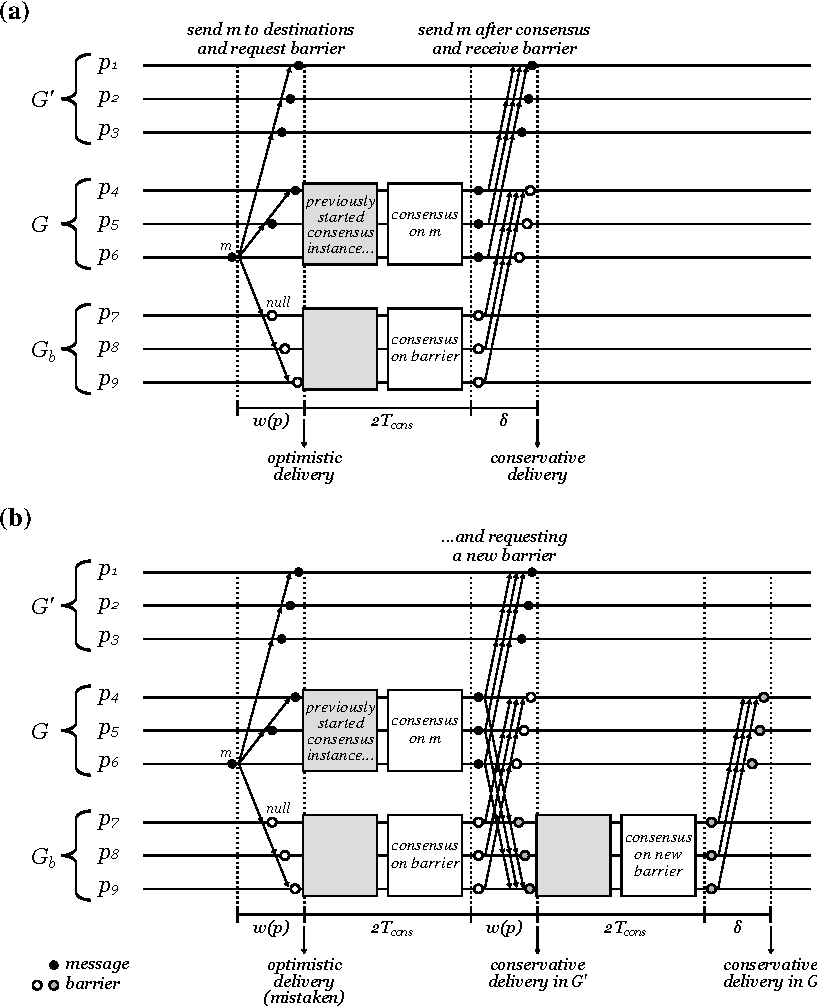
\includegraphics[width=0.8\linewidth]{images/optdel}
  \caption{Execution examples when the optimistic assumption holds (a) and when it fails to hold (b)}
  \label{fig:optdel}
\end{figure}

% 
% \begin{algorithm}
% \begin{distribalgo}[1]
% 
% \blankline
% \INDENT {Initialization}
%   \STATE $k \leftarrow 0$, $nextProp \leftarrow 0$, $local\_decided \leftarrow \emptyset$, $local\_msgs \leftarrow \emptyset$, $optPending \leftarrow \emptyset$, $am-multicast \leftarrow \emptyset$
%   \INDENT{\textbf{for all} $G' \in sendersTo(G)$ \textbf{do}}
%     \STATE $barrier(G',G) \leftarrow -\infty$ 
%   \ENDINDENT
% \ENDINDENT 
% 
% \blankline
% \INDENT{\textit{To send a message $m$} -- \amcastarg{m}}
%   \STATE $m.ts \leftarrow getTime()$  
%   \COMMENT{current wallclock value as the timestamp of $m$}
%   \STATE \rmcastarg{$m$}{$m.dst \cup \{G\} \cup blockers(m)$}
% %  \INDENT{\textbf{for all} $p' \in m.dst \cup \{G\} \cup blockers(m)$ \textbf{do}}
% %    \STATE send($p'$, $m$)    
% %    \COMMENT{send optimistically $m$ to all involved processes}
% %  \ENDINDENT
% \ENDINDENT
% 
% \blankline
% \INDENT{\textit{When} \rmdelarg{$m'$}}
%   \IF {$G \neq m'.src$ $\wedge$ $\exists G' \in (m'.dst \cap receiversFrom(G))$}
%     \STATE $null \leftarrow$ empty message
%     \STATE $null.src \leftarrow G$  \COMMENT{some other group needs a barrier from this one}
%     \STATE $null.ts \leftarrow m'.ts$ \label{algline:nulltsmts}
%     \STATE $null.dst \leftarrow m'.dst \cap receiversFrom(G)$
%     \STATE $optPending \leftarrow optPending \cup \{null\}$
%   \ENDIF
%   \IF {$m'.ts < getTime() - w(p) \vee G \notin m'.dst$}
%     \STATE discard $m'$
%     \COMMENT{late commands probably lead to out-of-order delivery}
%   \ELSE
%     \STATE $optPending \leftarrow optPending$ $\cup$ $\{m'\}$
%   \ENDIF
% \ENDINDENT
% 
% \blankline
% \INDENT{\textit{When $\exists m \in optPending : getTime() > m.ts + w(p)$ $\wedge\ \nexists m' \in optPending: m'.ts < m.ts$}}
%   \STATE $optPending \leftarrow optPending \setminus \{m\}$
%   \IF {$G \in m.dst \wedge m \neq null$}
%     \STATE \optdel{$m$}  
%   \ENDIF
%   \IF {$G = m.src$}
%     \STATE $local\_msgs \leftarrow local\_msgs \cup \{m\}$
%   \ENDIF
% \ENDINDENT
% 
% \blankline
% \INDENT{\textit{When $\exists m \in local\_msgs \wedge nextProp = k$}}
% %  \STATE $local\_msgs \leftarrow local\_msgs \setminus \{m\}$
% %  \IF {$m \notin local\_decided \wedge \nexists m' \in local\_decided: m'.ts > m.ts$}
%     \STATE $local\_msgs \leftarrow local\_msgs \setminus (local\_decided \cup \{m' : \exists m'' \in local\_decided \wedge m'.ts < m''.ts \wedge m' \neq null\})$ \label{algline:keepnull}
%     \IF {$local\_msgs \neq \emptyset$}
%       \STATE $nextProp \leftarrow k + 1$
%       \STATE Propose($k$,$local\_msgs$)
%     \ENDIF
% %  \ENDIF
% \ENDINDENT
% 
% \blankline
% \INDENT{\textit{When} Decide($k$,$msgSet$)}
% %  \STATE $m.gs \leftarrow k$
%   \STATE $local\_decided \leftarrow local\_decided \cup msgSet$
%   \INDENT{\textbf{for all} $m \in msgSet : G \in m.dst \wedge m \neq null$ \textbf{do}} \label{algline:checkcons}
%     \STATE $am-multicast \leftarrow am-multicast \cup \{m\}$
%   \ENDINDENT
%   \INDENT{\textbf{while} $\exists m \in msgSet : (\forall m' \in msgSet : m \neq m' \Rightarrow m.ts < m'.ts)$ \textbf{do}}
%     \INDENT{\textbf{for all} $p' \in m.dst \setminus \{G\}$ \textbf{do}}
%       \STATE send($p'$, $\{m, \text{`cons'}\}$)
%       \COMMENT{this message is sent through a FIFO lossless channel}
%     \ENDINDENT
%     \STATE $msgSet \leftarrow msgSet \setminus \{m\}$
%     \COMMENT{the messages are sent in ascending order of timestamp}
%   \ENDINDENT
%   \STATE $nextProp \leftarrow k + 1$
%   \STATE $k \leftarrow k + 1$  
% \ENDINDENT
% 
% \blankline
% \INDENT{\textit{When} receive($\{m',\{\text{`cons'}\}$)}  
%   \IF {$m' \notin\ am-multicast \wedge m' \notin\ delivered \wedge m' \neq\ null$}
%     \STATE $am-multicast \leftarrow am-multicast \cup \{m\}$
%   \ENDIF
%   \STATE $barrier(m'.src,G) \leftarrow max(m'.ts, barrier(m'.src,G))$  \COMMENT{channels are FIFO, but there are different senders}
% \ENDINDENT
% 
% \blankline
% \INDENT{\textit{When $\exists m \in am-multicast : \forall G' \in sendersTo(G): m.ts < barrier(G',G)$\\ $\wedge\ \nexists m' \in am-multicast : m'.ts < m.ts$ }}
%   \STATE $am-multicast \leftarrow am-multicast \setminus \{m\}$
%   \STATE \consdel{$m$}
%   \STATE $delivered \leftarrow delivered \cup \{m\}$
% 
% \blankline
% \ENDINDENT
% 
% \caption{\amcastarg{m} -- executed by every process $p$ from group $G$}
% \label{algorithm:nullondemand}
% \end{distribalgo}
% \end{algorithm}



\subsection{Parallel instances of consensus}
\label{sec:parallel}

We can further optimize the delivery algorithm. One major problem with proposing messages with consensus is that the previous algorithms wait until a consensus instance has been finished to start a new one, so that no message is proposed twice. However, even if a message is proposed and accepted twice, each process may choose to consider only the first time (i.e. the consensus instance with lowest id) when a message $m$ has been proposed. This would require some more local processing and could cause some unnecessary traffic due to messages being proposed in different consensus instances. The worst case delivery time of a message $m$, when using the optimistic delivery and barrier requests, would be $2w(p) + 2\tconsm + \delta$. It must be noted, however, that this represents the case when the optimistic assumption fails to hold and $m$ has its timestamp changed. Otherwise, the conservative delivery time would be $w(p) + \tconsm + \delta$.

The basic idea would be that, whenever a process $p$ has a pending message $m$ that it received, it will propose it in some instance $I$ as soon as its clock has a value greater than $m.ts.rtc + w(p)$. As $p$ cannot foresee whether $m$ will be decided in $I$ or not, it keeps the double $(m,I.id)$ in a $trying$ list. When $I$ terminates, $(m,I.id)$ is removed from $trying$ and $p$ checks whether $m$ has been decided -- which might have happened also in some instance $I' \neq I$ in the meantime -- by checking its $local\_decided$ list. If not, $p$ proposes $m$ again in some consensus instance $I''$ and inserts $(m,I''.id)$ into $trying$.

Even if the consensus instances are run in parallel, we consider that they make a callback to \emph{Decide()} in ascending order of instance id. This can be easily done by the consensus implementation using a sequence number. Whenever a message $m$ is agreed upon in some consensus instance $I$, any later decision of $m$ in some instance \mbox{$I' : I'.id > I.id$} is merely ignored.



\subsection{Using Paxos with a leader for consensus}
\label{sec:paxos}

Although ensuring termination of consensus in an asynchronous system is not possible \cite{fischer1985idc}, the Paxos \cite{lamport1998ptp} algorithm can guarantee the termination of an instance $I$ as long as some assumptions are held:

\begin{itemize}
  \item the maximum message delay bound $\delta$ is known;
  \item at some point in the execution of $I$, there is a leader which does not fail until a value has been chosen\footnote{Lamport demonstrates in \cite{lamport1998ptp} that, if the time needed to elect a leader is $T_{el}$, the time needed to conclude a consensus instance would be at most $T_{el} + 9\delta$ after the last leader failure during the execution of $I$.};
  \item during the whole execution of $I$, more than half of the processes are correct, that is, if the number of faulty processes is $f$ and the total number of processes is $n$, $f < \lceil \frac{n}{2} \rceil$;
  \item enough messages are successfully received, that is, for each phase of the execution of $I$, a majority of processes succesfully receive the leader's message or the leader successfully receives the reply (be it a confirmation or a negative acknowledgement) from a majority of processes.
\end{itemize}

Paxos uses the abstraction of \emph{proposers}, \emph{acceptors} and \emph{learners}. In short, the acceptors are the processes which have to agree upon some value given by the proposers. The learners are those who are notified about which value has been accepted. With a leader, Paxos can achieve consensus in most instances, except the first one since the last leader change, in $3\delta$ -- forwarding a proposal to the leader, sending it to the other processes (acceptors) and receiving a confirmation. Each acceptor can send the confirmation to every learner, so that each learner can figure out by itself that a value has been agreed upon once it receives a confirmation from a majority of acceptors.

In the context of our \amcast{} primitive, the first communication step of Paxos -- forwarding a message $m$ to the leader -- is already done by means of \rmcast{}ing each message to a set of processes that includes every process in $m$'s group of origin. The last phase, which consists of every learner receiving the confirmation of a majority of acceptors, can also include the $\delta$ contained in the conservative message delivery time we analysed before: instead of waiting for a message to be decided and only then notifying other groups, the acceptors of a group can also send the confirmation to processes in other groups, so that also they can infer the first group's decision right away. This implies that, for each consensus instance run within a group $G$, each process in the groups of $receiversFrom(G)$ would be a learner for that instance. Figure \ref{fig:paxosmanylearnergroups} illustrates this: process $p_1$ from group $G$, whose leader is $p_3$, \amcast{}s $m$; in the last phase of the consensus protocol, the processes in $G' \in receiversFrom(G)$ receive the confirmation message from the acceptors of $G$, so no extra communication step is needed to notify them about the final timestamp of $m$.

As $m$ was \rmcast{} in the beginning, there is no need to send all of its contents again in the consensus instance. Instead, only the timestamp of $m$ is proposed, since this is the information that must be agreed upon -- and which may change if the optimistic assumption does not hold and some other message of higher timestamp is delivered before $m$. In any case, as all messages agreed upon in $G$ are notified to $G'$, also the processes of $G'$ are able to infer the final timestamp of each message from $G$.

As we are making an optimistic assumption -- that each $p$ waits for a time $w(p)$ long enough so that no timestamps must be changed -- for the message delivery, the barriers are being requested to other groups in parallel, since $m$ is also \rmcast{} to $blockers(m)$ in the first communication step of our protocol. If such assumption holds, the barriers received will have a greater timestamp than $m$ and, thus, the conservative delivery of $m$ will take place $w(p) + 2\delta$ after it has been sent. If the clocks are perfectly synchronized and $w(p)$ does correspond to the maximum interprocess communication delay $\delta$, the time needed to conservatively deliver a message using this algorithm would be $3\delta$.

Finally, we can guarantee a conservative delivery time of $3\delta$, if no message had its timestamp changed, because the barrier requests for that message were made based on its initial timestamp. If the timestamp has changed, then a new barrier request may have to be made to ensure the delivery of that message. Unfortunately, to guarantee the delivery of the message, such request can be done only after the final timestamp has been decided: once the source group of a message $m$ noticed a change in $m.ts$, it sends another barrier request to $blockers(m)$. This request is handled in a way very similar to a conservative delivery, in the sense that, once it is received by a process, a null message is proposed, decided and then sent back to the destinations of $m$. This would take extra $3\delta$, so the worst case conservative delivery time would be $6\delta$.

Note, however, that for this worst case scenario to happen it would be necessary for the leader $p$ of group $G$ to: (1) not know some value greater than or equal to $w(p)$; (2) have received and proposed some message $m' : m'.ts > m.ts$ before $m$ and (3) not have received any barrier with value greater than the new timestamp of $m$. Even after changing the timestamp of $m$, it may be not necessary to request a new barrier from each group in $sendersTo(G)$, because some other barrier -- possibly requested because of some other message -- with a value higher than the new timestamp of $m$ may have been received already.

\begin{figure}
  \centering
  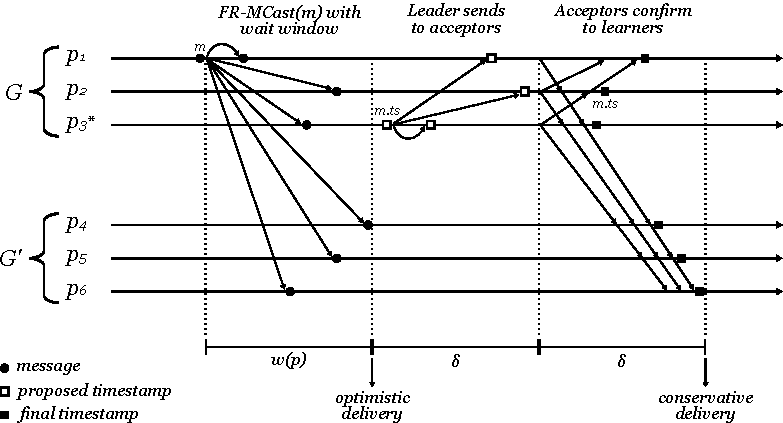
\includegraphics[width=0.8\linewidth]{images/paxos3d}
  \caption{Deciding the final timestamp and notifying other groups in three communication steps}
  \label{fig:paxosmanylearnergroups}
\end{figure}



\subsection{Relaxing validity and discarding stale messages}
\label{sec:discard}

Although unlikely to happen, the worst case delivery time of \amcast{} when using Paxos with a leader for consensus and requesting barriers in the beginning of the protocol is $6\delta$. It is so because some messages may need to have their initial timestamp changed as a possible consequence of the optimistic assumption \emph{A2} not holding. However, a simple way to eliminate the possibility of having to change timestamps is by not considering messages whose delivery order does not follow the order of the initial timestamps.

Although discarding messages which do not follow the initial timestamp order conflicts with the properties we have defined for the \amcast{} primitive, we describe it here because then every message would be delivered within $3\delta$, in the worst case. The validity property would now be changed to:

\textbf{Optimistic Uniform Validity}: if a process \amcast{}s $m$ and the optimistic assumption \emph{A2} holds, then one of the correct processes that is a destination of $m$ eventually \cons{}s $m$.

The problem with changing the original uniform validity property is that it could make the multicast primitive impracticable for some applications. Nevertheless, some other applications not only do not require messages to be delivered if they arrive out of order, but also it is better not to deliver such messages at all -- such as real-time streams of audio or video or online real-time multiplayer games.


\section{Proof of correctness}
\label{sec:proofs}

Here, we prove that the \amcast{} primitive ensures the properties defined in section \ref{sec:model} -- uniform validity, uniform agreement, uniform integrity, uniform total order and FIFO order. To do this, we prove that Algorithm \ref{algorithm:deliveryminimal}, when used along with Algorithm \ref{algorithm:nullperiodic}, ensures these properties.

\subsection{Uniform Validity}

\subsection{Uniform Agreement}

\subsection{Uniform Integrity}

This property means that, if a message $m$ was delivered to process $p$ of group $G$, then it has (1) been multicast before, (2) $G \in m.dst$ and (3) it has not been delivered by $p$ before.

For a message $m$ to be delivered (l. \ref{algline:consdeliver}), it must be contained in the $am-multicast$ list (from the condition in line \ref{algline:inam-multicast}).  There are two possibilities to when $m$ has been inserted into such list:
\begin{itemize}
  \item $m$ has been originated in the same same group of $p$, that is, $p \in m.dst$, which means $m$ was inserted into $am-multicast$ in line \ref{algline:insbp2} of Algorithm \ref{algorithm:deliveryminimal}, or
  \item $m$ has been sent from a group $G \neq G'$, which means that it was inserted into $am-multicast$ in line \ref{algline:insbp1}. 
\end{itemize}

In line \ref{algline:insbp2}, $m$ is inserted into $am-multicast$ only if $G \in m.dst$, which satisfies condition (2), and if it was decided in some consensus instance within $G$. To have been decided within $G$, from the properties of consensus \cite{lamport1998ptp}, we know that it must have been proposed by some process of $G$, which happens in line \ref{algline:propose}. In line \ref{algline:propose}, for a message to be proposed, it must be in the $local\_msgs$, as its contents are the value proposed. For a message to be in the $local\_msgs$ list, it must have been inserted there, which happens only in line \ref{algline:addtogroupmsgs}. For l. \ref{algline:addtogroupmsgs} to be executed, $m$ must have been \rmdel{}ed and $G$ must be the source group of $m$, that is, $m.src = G$. For a message to be \rmcast{} by a process to its own group, a \amcastarg{$m$} call must have been made -- which satisfies condition (1) --, for line \ref{algline:rmlocal} is the only one where a process \rmcast{}s a message to its own group. 

Also, for a message to be inserted into $local\_msgs$ (l. \ref{algline:addtogroupmsgs}) it cannot have been decided already (l. \ref{algline:removedecided}). We assume here that a process can only make a proposal for consensus instance $k$ when it knows all the values decided in all instances prior to $k$. Therefore, when a process proposes a message, it knows all the messages which were already decided in previous consensus instances. As a decided message is inserted into a $local\_decided$ list (l. \ref{algline:addtodecided}, which is always executed after a decision), a process cannot propose a message which was decided already and, therefore, a message cannot be decided twice (in two different consensus instances). As a message is inserted into $am-multicast$ by processes of its own group of origin only when decided (l. \ref{algline:insbp2}), it cannot be inserted twice, thus it cannot be delivered twice, satisfying condition (3).

As for processes from destination groups which are not from the source group of $m$, they will never execute line \ref{algline:insbp2}, since they never decide on $m$. However, processes of the group $m.src$, which is the source of $m$, will \rmcast{} $m$ to every $G'$ which is a destination of $m$ other than $G$ (l. \ref{algline:rmothers}). When a process in $G'$ \rmdel{}s $m$, it checks whether $m$ was already inserted into $am-multicast$ or $delivered$, where $delivered$ is the list of all messages which were ever \amdel{}ed. Once a message has been inserted into \mbox{$am-multicast \cup delivered$}, it stays there forever -- a message is only removed from $am-multicast$ in line \ref{algline:rmfrombp}, right after what it is then inserted into $delivered$, in line \ref{algline:addtodelivered}. Therefore, also messages which arrive from other groups are never inserted twice into $am-multicast$. As each message is removed from $am-multicast$ right before being \amdel{}ed, it is never delivered twice, satisfying (3).

For line \ref{algline:insbp1}, $m$ is inserted into $am-multicast$ of process $p'$ of group $G'$ when it has been \rmdel{}ed, and only if $m.src \neq G'$. For a process $p \in G \neq G'$ to \rmcast{} $m$, $m$ must have been decided within $G$, which means that it was proposed within $G$, therefore it was \amcast{} -- satisfying condition (1) -- by $G \neq G'$ to $G'$, which, from line \ref{algline:rmothers}, necessarily belongs to $m.dst$, satisfying condition (2).

Finally, as for Algorithm \ref{algorithm:nullperiodic}, $null$ messages are never delivered, so they will never violate the uniform integrity property.

\begin{flushright}
$\square$
\end{flushright}

\subsection{Uniform Total Order}

\subsection{FIFO Order}

\section{Related work}

\cite{sousa2002oto}: optimistic total order bcast in wans: for the opt-delivery to work properly, requires that the delay between each pair of processes stay constant (ours only requires that it never goes beyond $w(p)$ for each process $p$\ldots). sequencer based (no tolerance for failures of the sequencer). not mentioning multicast.

\section{Experimental results}

\section{Conclusion}

%\bibliographystyle{latex8}
%\bibliography{main}
\bibliographystyle{acm}
\bibliography{gftommog}
\end{document}

